%% WRITTEN & DESIGNED BY AFONSO MONIZ MOREIRA IN 4/02/2020
%% 

%The beamer (presentation) document type
\documentclass[10,5pt, pdf]{beamer}
\setbeamersize{text margin left=5mm,text margin right=5mm}%Modificar as margens do Beamer

%The usual packages apply:

%For languages beside English:
\usepackage[portuguese]{babel}

%For typing accents
\usepackage[utf8]{inputenc}
%For hypenation
\usepackage[T1]{fontenc}

% Beamer Properties
\usepackage{enumerate}
\setbeamertemplate{frametitle continuation}{} %Removing Frame Roman Numbering
\usefonttheme{serif}
\renewcommand\sfdefault{cmbr}
\setbeamertemplate{theorems}[numbered] %Theorem, Proof, Definitions, Lemma
\beamertemplatenavigationsymbolsempty %Remove os simbolos de navegação
\usepackage{beamerthemesplit}
\usetheme{Boadilla}
\usecolortheme{beaver}

% For Tables
\usepackage{booktabs}
\usepackage{adjustbox}
\usepackage{tabls}
\usepackage{xcolor}


% Figures
\usepackage{graphicx}
\graphicspath{{G:/My Drive/academia_drive/actividade_docente/ano_lectivo_2023_2024/estatistica_II/slides_das_aulas_teróricas/aulas_de_teste_de_hipoteses/figures}}% For specifying a different path for the figures
\usepackage{epstopdf} % Converts EPS to PDF
\usepackage{pdfpages} % Inserting a PDF in Document
\usepackage{tcolorbox}
\usepackage{tikz}
\usepackage{pgfplots}
\pgfplotsset{compat=1.17}

% for math
\usepackage{amsmath}
\usepackage{nccmath}%Aligning equations to the left
\usepackage{amssymb}
\usepackage{cancel}
\usepackage{pgfplots}
\pgfplotsset{compat=1.17} % Ensure compatibility with your pgfplots version

\pgfplotsset{compat=newest}
\usepackage{etoolbox}
\AtBeginEnvironment{equation}{\scriptsize} %all equation enviroments have a given letter size

% for code
\usepackage{listings}
\usepackage{xcolor} % For custom colors


% for including Programming Code
%\usepackage[]{listings}% General Code
%\usepackage[numbered]{mcode}% Matlab Code

%for Proof enviroment
\usepackage{amsthm}

%for Bibliography
\usepackage{natbib}

%%%%%%%%%%%%%%%%
%Title Page Info
%%%%%%%%%%%%%%%%
\title{Estatística II}
\subtitle{Teste de Hipóteses}
\institute{Departamento de Métodos Quantitativos para a Economia e Gestão (DMQEG)}
\author{Afonso Moniz Moreira}
\date{2º Semestre - 2023-2024}

%%%%%%%%%%%%%%%%
\begin{document}
%%%%%%%%%%%%%%%%


%%%%%%%%%%%%%%%%
%Title Page 
%%%%%%%%%%%%%%%%
{
\usebackgroundtemplate{%
\tikz[overlay,remember picture] \node[anchor=north, inner sep=12pt] at (current page.north) {
\includegraphics[height=1.55cm]{iscte_business_school_logo.png}}; % Adjust height and path as needed
}
\begin{frame}[plain]
\vspace{0.5cm}
\textbf{}\\
\footnotesize{}
\vspace{1cm}
\titlepage
\end{frame}
}


%%%%%%%%%%%%%%%%
% FRAME
%%%%%%%%%%%%%%%%
\begin{frame}{Attention this is not a test!}{Disclaimer}
\begin{center}
Este conjunto de slides não pretendem, nem conseguem, substituir a leitura \textbf{atenta} da bibliografia principal da cadeira.\par
\pause
O objetivo dos mesmos é apenas guiar as aulas teórico-práticas de estatística II.\par
\pause
Neste sentido a qualquer momento podem ser abandonados de forma discricionária pelo docente da cadeira, especialmente se os slides incentivarem os alunos a comportamentos não exemplares.\par
\pause
Como  por exemplo o aumento acentuado do nível de decibéis (Db) dentro da sala de aula. 
\end{center}
\end{frame}
%%%%%%%%%%%%%%%%
%%%%%%%%%%%%%%%%


\section{Teoria dos Ensaios de Hipóteses}\label{sec:ex1}
%%%%%%%%%%%%%%%%
% FRAME
%%%%%%%%%%%%%%%%
\begin{frame}{Teoria dos Ensaios de Hipóteses}{Qual é a utilidade ?}
\begin{itemize}
    \item{Para que serve um ensaio de hipóteses ?}
    \begin{itemize}
    \pause
        \item{Servem para credibilizar ou descredibilizar afirmações.}
        \pause
        \item{Então... mas nós conseguimos fazer isso com os intervalos de confiança...}
        \pause
        \item{Verdade, mas não com o nível de granularidade (ou precisão) de um teste de hipóteses.}
    \end{itemize}
    \pause
\item{Que tipo de perguntas conseguimos responder?}
\pause
\begin{itemize}
\pause
    \item{''O Ministério da Saúde afirma que, com os meios agora postos à disposição dos hospitais civis, o número médio de dias de internamento é, no máximo, oito.''}
    \pause
    \item{Seja $X\equiv$ Número de dias que um doente fica internado no hospital.}
    \pause
    \item{$X \sim \mathcal{N}(\mu, \sigma)$, assumindo uma população normal.}
    \pause
    \item{Portanto, matematicamente, será que $\mu=8$ ?}
\end{itemize}

\end{itemize}
\end{frame}
%%%%%%%%%%%%%%%%
%%%%%%%%%%%%%%%%

%%%%%%%%%%%%%%%%
% FRAME
%%%%%%%%%%%%%%%%
\begin{frame}{Teoria dos Ensaios de Hipóteses}{Qual é a utilidade ?}
\begin{itemize}
\item{Uma outra situação:}
\pause
\begin{itemize}
    \item{''Pretendem comparar-se dois processos de fabrico do mesmo produto.
Adopta-se a seguinte regra de decisão: com base numa amostra de 100
unidades para cada processo, eliminar-se-á aquele processo que conduza a uma proporção observada de produtos defeituosos superior à do outro, em pelo menos 2\%''}
\pause
\item{$Y_i\equiv$ Unidades defeituosas do processo de fabrico $i$, $i=\{1,2\}$}
\pause
\item{$Y_i \sim f(x|p)$, $p_i$ é a proporção de produto defeituosos.}
\pause
\item{Portanto, matematicamente, será que $p_1-p_2>0.02$ ou $p_2-p_1>0.02$ ?}
\end{itemize}
\pause
\item{São apenas dois exemplos onde os intervalos de confiança não conseguem responder com a mesma eficácia.}
\pause
\item{No entanto qualquer decisor (CEO, COO, CFO, CIO, CTO, etc) gostava de ter uma técnica para extrair a resposta a estas perguntas usando uma amostra aleatória.}
\end{itemize}
\end{frame}
%%%%%%%%%%%%%%%%
%%%%%%%%%%%%%%%%

\subsection{As Hipóteses e os Erros}\label{subsec:hiperros}
%%%%%%%%%%%%%%%%
% FRAME
%%%%%%%%%%%%%%%%
\begin{frame}{As Hipóteses e os Erros}{Quais são as hipóteses ?}
\begin{itemize}
    \item{Considerem um tribunal em que uma dada acusação é credibilizada ou descredibilizada mediante a apresentação de provas de por parte da defesa e da acusação e no final o juiz decide.}
    \pause
    \item{Um ensaio de hipóteses inspira-se na mesma envolvência com umas diferenças:}
    \pause
    \begin{itemize}
        \item{A prova é a amostra aleatória.}
        \pause
        \item{O juiz é o teste estatístico que foi escolhido.}
    \end{itemize}
    \pause
    \item{Assim sendo iremos ter duas hipóteses:}
    \begin{itemize}
        \pause
        \item{$H_0$ - A hipótese nula é a presunção de inocência de um réu.} 
        \pause
        \item{$H_1, H_a$ - A hipótese alternativa é a contraposição da anterior.} 
    \end{itemize}
    \pause
    \item{Quando os dados da amostra (i.e as provas) são usadas numa determinada formulação de teste (i.e o juiz) podemos ter os seguintes resultados:}
\end{itemize}
\end{frame}
%%%%%%%%%%%%%%%%
%%%%%%%%%%%%%%%%

%%%%%%%%%%%%%%%%
% FRAME
%%%%%%%%%%%%%%%%
\begin{frame}{As Hipóteses e os Erros}{Os Erros Possíveis}
\begin{itemize}
    \item{Os dados fornecidos (i.e as provas) ao teste formulado (i.e o juiz) \textbf{não levam} a uma \textbf{rejeição} da hipótese nula (i.e do status quo).} 
    \pause
    \item{Os dados fornecidos (i.e as provas) ao teste formulado (i.e o juiz) \textbf{levam} a uma \textbf{rejeição} da hipótese nula (i.e do status quo).} 
    \pause
    \item{Qual é a diferença entre o não rejeitar e o aceitar ?}
    \pause
    \item{Tal e qual como num julgamento podem existir erros...}
    \pause
    \item{Um instrumento de avaliação comum em vários domínios da estatística é a matriz de confusão.}
\end{itemize}
\end{frame}
%%%%%%%%%%%%%%%%
%%%%%%%%%%%%%%%%

%%%%%%%%%%%%%%%%
% FRAME
%%%%%%%%%%%%%%%%
\begin{frame}{As Hipóteses e os Erros}{Erro tipo I e tipo II}

\begin{table}
\centering
\begin{tabular}{c|c|c|}
\cline{2-3}
& \multicolumn{2}{c|}{Situação Real (i.e. Observada)} \\ 
& $H_0$ Verdadeira & $H_0$ Falsa \\ \hline
\multicolumn{1}{|c|}{\begin{tabular}[c]{@{}c@{}}Rejeita\\ $H_0$\end{tabular}} & \textcolor{red}{Erro do Tipo I (FN)} & Decisão Correcta (VP) \\ \hline
\multicolumn{1}{|c|}{\begin{tabular}[c]{@{}c@{}}Não Rejeita\\ $H_0$\end{tabular}} & Decisão Correcta (VN) & \textcolor{blue}{Erro do Tipo II (FP)} \\ \hline
\end{tabular}
\end{table}
\pause
\begin{itemize}
    \item{Erro Tipo I - A Hipótese nula \textbf{é rejeitada} quando, de facto, é verdadeira. - O réu é injustamente condenado.}
    \pause
    \item{Erro Tipo II - A Hipótese nula \textbf{não é rejeitada} quando, de facto, é falsa. - o réu é injustamente ilibado.}
    \pause
    \item{Cada vez que um ensaio de hipóteses é executado os dois erros estão presentes e devem ser controlados.}
\end{itemize}

\end{frame}
%%%%%%%%%%%%%%%%
%%%%%%%%%%%%%%%%

\subsection{Execução de Um Ensaio de Hipóteses}
%%%%%%%%%%%%%%%%
% FRAME
%%%%%%%%%%%%%%%%
\begin{frame}{Execução de Um Ensaio de Hipóteses}{Passos Necessários - Problema Exemplo}
\begin{itemize}
    \item{Seguindo \cite{reis2019a} vamos considerar um exemplo para delinear os passos necessários.}
    \pause
    \item{''Uma pizzaria recebe diariamente encomendas por telefone, que se têm comportado segundo uma lei normal. A empresa está dimensionada para uma procura média diária que não ultrapasse as 200 pizzas, admitindo um desvio-padrão de 15. Uma campanha promocional realizada nos últimos 9 dias levou a uma procura média de 210 pizzas. O problema consiste em avaliar a necessidade de reforçar a capacidade média de venda, estudando se houve de facto uma alteração significativa na procura média diária de pizzas''}
\end{itemize}
\end{frame}
%%%%%%%%%%%%%%%%
%%%%%%%%%%%%%%%%

%%%%%%%%%%%%%%%%
% FRAME
%%%%%%%%%%%%%%%%
\begin{frame}{Execução de Um Ensaio de Hipóteses}{Passo I - Definir as Hipóteses}
\begin{itemize}
    \item{Existiu uma quebra de estrutura na procura ? Ou seja tenho de redimensionar a minha loja ?}
    \begin{itemize}
        \pause
        \item{Considere-se $X\equiv$ Procura diária de pizzas no estabelecimento.}
        \pause
        \item{Sabe-se que $X\sim \mathcal{N}(\mu, \sigma=15)$. Queremos perceber se $\mu$ se alterou.}
    \end{itemize}
    \pause
    \item{Deste modo queremos que os dados respondam a isto:}
    \begin{itemize}
        \pause
        \item{$H_0: \mu \leq 200$ V.S $H_1: \mu > 200$ - Teste Unilateral}
        \pause
        \item{Portanto queremos saber se a procura média se estabeleceu num novo patamar pelo que o COO tem de propor ao board um aumento da capacidade da pizzaria.}
    \end{itemize}
    \item{Como vamos ver existem várias formulações de hipóteses.(i.e Testes)}
    \pause
    \item{Unilateral $\Rightarrow$ Sinal da alteração $\Rightarrow$ $H_a (< ou >)$ $H_0 (=, \leq ou \geq)$.}
    \item{Bilateral $\Rightarrow$ $\Delta$ face a um valor concreto $K$ $\Rightarrow$ $H_a (\neq)$ $H_0(=)$.}
\end{itemize}
\end{frame}
%%%%%%%%%%%%%%%%
%%%%%%%%%%%%%%%%

%%%%%%%%%%%%%%%%
% FRAME
%%%%%%%%%%%%%%%%
\begin{frame}{Execução de Um Ensaio de Hipóteses}{Passo II - Definir o nível de significância $\alpha=1-\lambda$}
\begin{itemize}
    \item{Temos de definir um nível de significância do teste $\alpha$ que se liga diretamente com o nível de confiança que já viram nos ICs.}
    \pause
    \item{Estabelece o limite para a região de aceitação (RA) e para a região crítica ou de rejeição (RC)}
    \pause
    \item{O nível de significância impõe um trade-off à decisão ? Sim}
    \pause
    \item{O mais standard será $\alpha=0.05$, normalmente os papers que fazem uso de um teste de hipóteses mostram a decisão com 3 níveis de significância: 1\% (***), 5\%(**), 10\%(*) e $>10\%$ ().}
\end{itemize}
\end{frame}
%%%%%%%%%%%%%%%%
%%%%%%%%%%%%%%%%


%%%%%%%%%%%%%%%%
% FRAME
%%%%%%%%%%%%%%%%
\begin{frame}{Execução de Um Ensaio de Hipóteses}{Passo III - Escolha da Estatística Adequada ao Ensaio.}
\begin{itemize}
    \item{Como é que se escolhe a estatística de teste adequada ?}
    \begin{itemize}
        \pause
        \item{Em linha com os ICSs, vai depender do que sabemos (i.e. do setup estatístico) - tipo de população e respetivos parâmetros e dimensão da amostra.}
        \pause
        \item{Com base no ponto anterior e na definição das hipóteses escolhe-se uma estatística de teste que terá uma distribuição amostral conhecida.}
        \pause
        \item{No nosso caso concreto trata-se de um ensaio unilateral à média da população com variância conhecida pelo que a estatística adequada a todo este setup é:}
    \end{itemize}
    \pause
    \begin{equation}
        T=\frac{\bar{X} - \mu_0}{\frac{\sigma}{\sqrt{n}}}\sim \mathcal{N}(0,1)
    \end{equation}
    \pause
\item{Em avaliação vão ter um quadro, como nos ICs, onde vão puder escolher a melhor estatística para o teste que estão a executar.}
\end{itemize}
\end{frame}
%%%%%%%%%%%%%%%%
%%%%%%%%%%%%%%%%

%%%%%%%%%%%%%%%%
% FRAME
%%%%%%%%%%%%%%%%
\begin{frame}{Execução de Um Ensaio de Hipóteses}{Passo IV - Tomada de Decisão com uma Amostra Concreta}
\begin{itemize}
    \item{Então e agora como é que se decide para uma amostra concreta ?}
    \pause
    \item{Para o nível de significância do Passo II (i.e $\alpha=0.05$) calcula-se/calculam-se o/os valor/valores crítico/críticos da distribuição amostral:}
    \pause
    \item{O valor crítico em causa é $Z_{95\%}=1.645$ - \textbf{Ensaio à direita}.}
    \pause
    \item{Substitui-se os valores do nosso setup estatístico na estatística de teste:}
    \begin{equation}
        T^*=\frac{210 -200}{\frac{15}{\sqrt{9}}}=\frac{10}{5}=2.
    \end{equation}
    \pause
\item{O valor da estatística para a amostra concreta pertence à região crítica (RC): $\underbrace{2}_{T^*}\in\underbrace{[1.645,+\infty[}_{RC}$.}
\pause
\item{Os dados disponíveis não suportam a hipótese nula ($H_0$) então deve ser rejeitada.}
\pause
\item{A pizzaria deverá de facto aumentar a sua capacidade produtiva.}
\end{itemize}
\end{frame}
%%%%%%%%%%%%%%%%
%%%%%%%%%%%%%%%%


%%%%%%%%%%%%%%%%
% FRAME
%%%%%%%%%%%%%%%%
\begin{frame}{Execução de Um Ensaio de Hipóteses}{Passo IV - Tomada de Decisão com uma Amostra Concreta}
\begin{itemize}
    \item{Um outra maneira de avaliar o teste é calcular o valor crítico (i.e. o valor limite) para a estimativa associada ao parâmetro de interesse.}
    \pause
    \item{No nosso caso é $\mu$ e portanto trata-se de um valor limite à estimativa da média amostral $\bar{X}$.}
    \pause
    \begin{equation}
        \frac{\bar{X}_{\text{C}} - 200}{\frac{15}{\sqrt{9}}}=1.645\Longrightarrow \bar{X}_{\text{C}}=208.225
    \end{equation}
    \pause
    \item{Para não rejeitar a hipótese nula ($H_0$) a estimativa da média amostral teria de ter sido no máximo $\bar{X}_{\text{C}}=208.225$.}
    \pause
    \item{Contudo a amostra concreta deu origem a uma estimativa $\bar{X}=210$, pelo que a evidência estatística levam-me a rejeitar o status quo (i.e. $H_0$).}
\end{itemize}
\end{frame}
%%%%%%%%%%%%%%%%
%%%%%%%%%%%%%%%%

\section{Ex. Nº1}\label{sec:ex1}
%%%%%%%%%%%%%%%%
% FRAME
%%%%%%%%%%%%%%%%
\begin{frame}{Exercício Nº1 - Pág 163 de \cite{reis2021}}
\begin{itemize}
\item{''Um fabricante de baterias produz dois tipos de baterias, A e B cuja duração média é de 25 e 30 meses, respetivamente. O responsável pelo inventário viu-se confrontado com um lote de 100 baterias cujo tipo se desconhece. É sua convicção que o lote é do tipo A, o responsável decidiu proceder a um ensaio de hipóteses com base numa amostra de 4 baterias cuja duração média foi de 26,5 meses. Supondo que a duração das baterias segue uma distribuição normal com variância de 9 $meses^2$ o que é que se pode concluir ao nível da significância de $1\%$ ?''}
\pause
\item{Seja $X\equiv$ Duração, em meses, das baterias pertencentes ao lote não identificado.}
\pause
\item{$X\sim \mathcal{N}(\mu, \sigma=\sqrt{\sigma^2}=\sqrt{9}=3)$ - Normal com desvio-padrão conhecido.}


\end{itemize}
\end{frame}
%%%%%%%%%%%%%%%%
%%%%%%%%%%%%%%%%

%%%%%%%%%%%%%%%%
% FRAME
%%%%%%%%%%%%%%%%
\begin{frame}{Exercício Nº1 - Pág 163 de \cite{reis2021}}
\begin{itemize}
\item{Quais são as hipóteses que queremos verificar ?}
\pause
\item{$H_0:\mu=25$ (Convicção do Responsável) VS $H_1:\mu=30$}
\pause
\item{É um ensaio unilateral \textbf{à direita} à media populacional com desvio-padrão conhecido. (Valor de $H_1$ maior.)}
\pause
\item{Face aos dados que dispomos qual é a variável de teste  a utilizar ?}
\begin{itemize}
\item{Como a V.A $X\sim\mathcal{N}(\mu,\sigma)$ e $\sigma$ é conhecido então:}
\begin{equation}
T=\frac{\bar{X} - \mu_0}{\frac{\sigma}{\sqrt{n}}}\sim \mathcal{N}(0,1)
\end{equation}
\pause
\item{Para calcular o valor concreto da estatística de teste ($T^*$), substituímos o valor da amostra concreta:}
\pause
\begin{equation}
T^*=\frac{26.5 - 25}{\frac{3}{\sqrt{4}}}=1.    
\end{equation}
\pause
\end{itemize}
\item{A $\alpha=1\%$ de significância, o valor crítico da distribuição normal é $Z_{99\%}=2.326$ (ensaio à direita).}
\end{itemize}
\end{frame}
%%%%%%%%%%%%%%%%
%%%%%%%%%%%%%%%%

%%%%%%%%%%%%%%%%
% FRAME
%%%%%%%%%%%%%%%%
\begin{frame}{Exercício Nº1 - Pág 163 de \cite{reis2021}}
\begin{itemize}
\item{Assim sendo o valor de $T^*=1$ não ultrapassa o valor de $Z_{99\%}=2.326$, pelo que a evidência estatística não leva à rejeição da hipótese nula $H_0$.}
\pause
\item{$R.A=]-\infty, 2.326]$ e $R.C=[2.326, +\infty[$}
\end{itemize}
\pause
\begin{figure}
    \centering
    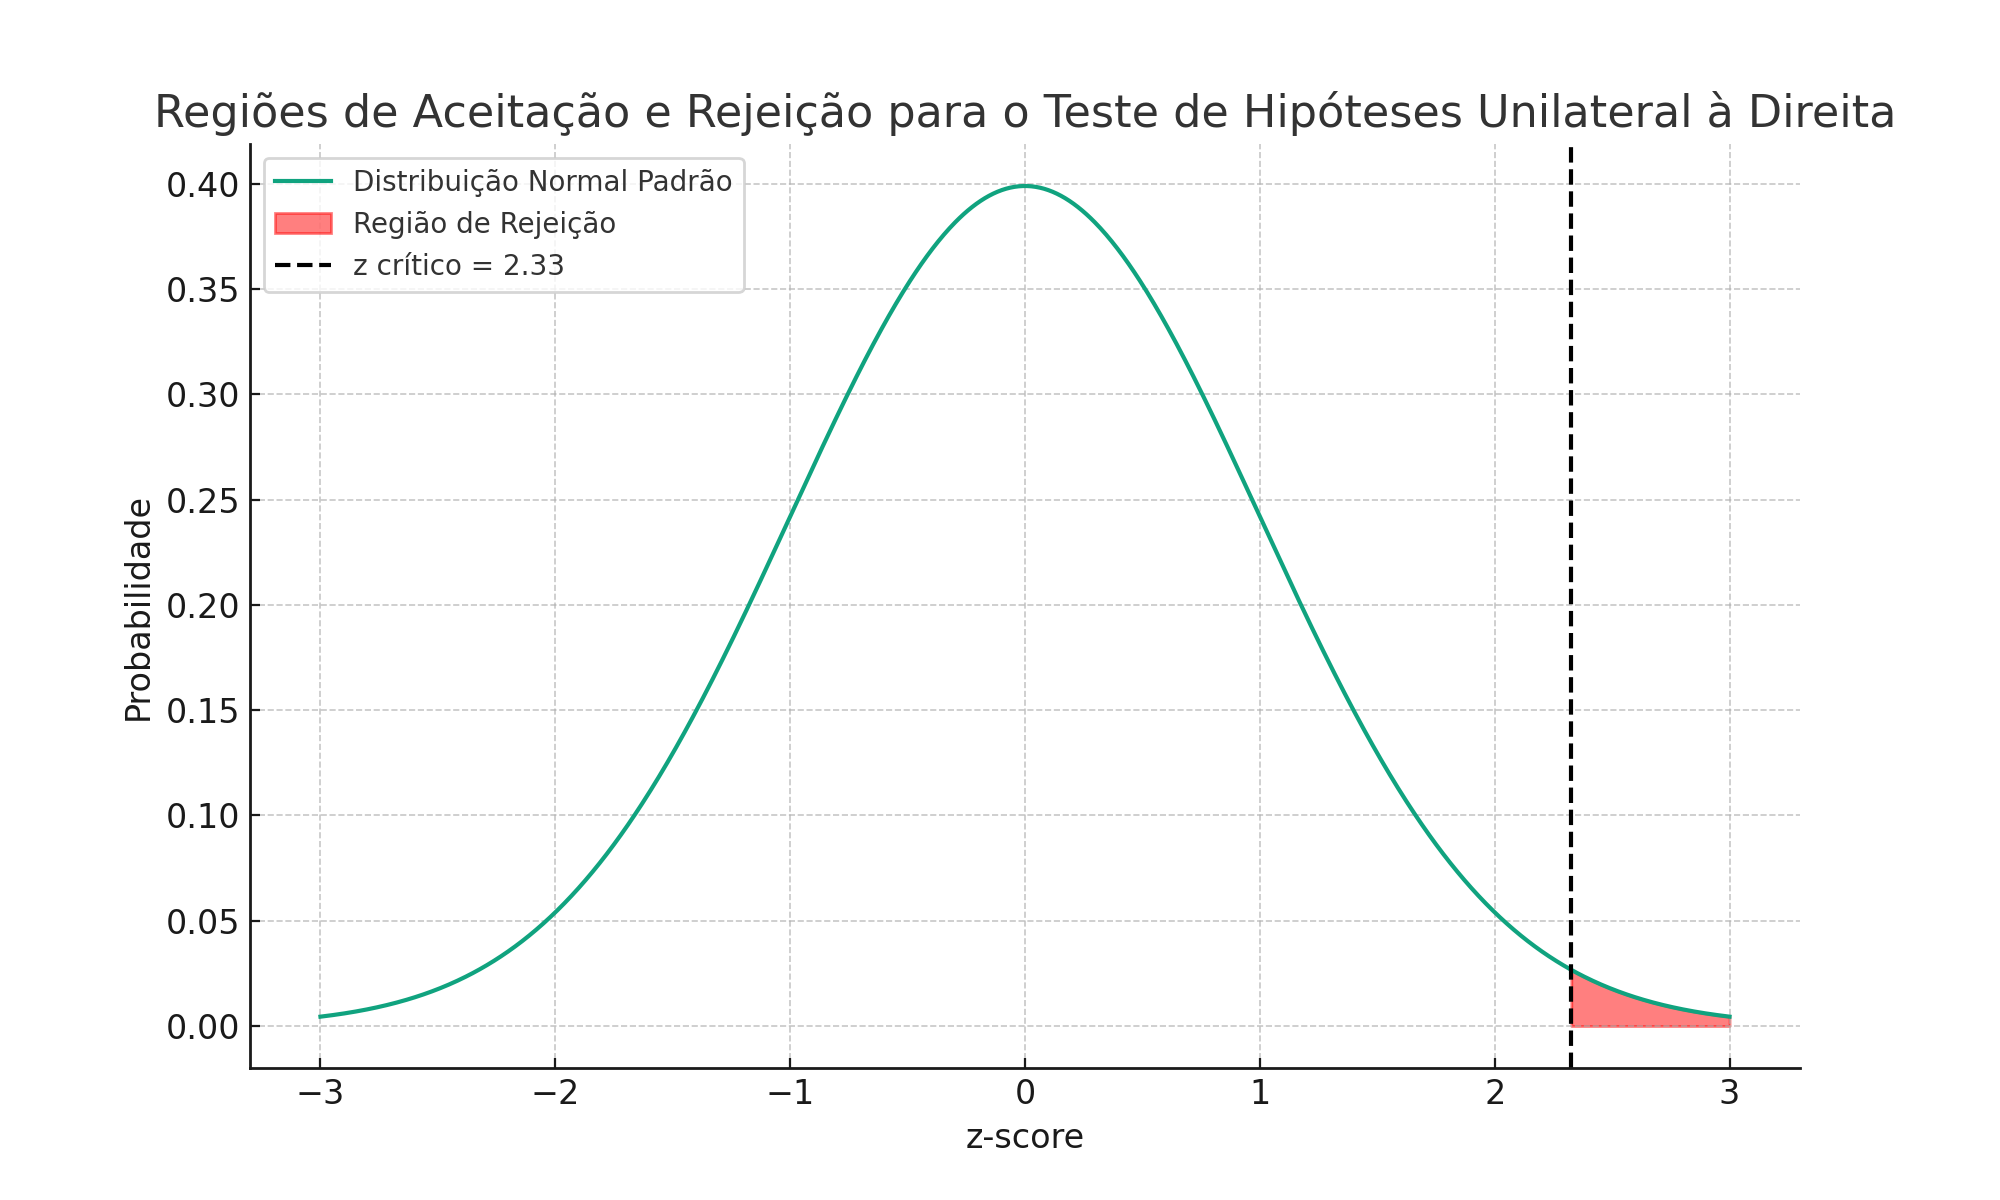
\includegraphics[scale=0.3]{ex1_plot.png}
    \caption{Região de aceitação e região crítica em termos de $Z$.}
\end{figure}
\end{frame}
%%%%%%%%%%%%%%%%
%%%%%%%%%%%%%%%%


\section{Ex. Nº4}\label{sec:ex4}
%%%%%%%%%%%%%%%%
% FRAME
%%%%%%%%%%%%%%%%
\begin{frame}{Exercício Nº4 -  Pág 164 de \cite{reis2021}}
\begin{itemize}
    \item{''Um fabricante de fitas magnéticas para computadores sabe que a resistência à rutura destas fitas é uma variável aleatória normalmente distribuída com média 300kg e desvio-padrão de 20Kg.''}
    \item{''Para ajuizar se uma nova técnica/processo de fabrico produz fitas em média mais fracas que as do processo antigo, foi usado o seguinte teste estatístico com um nível de significância de 5\% e um tamanho de amostra de $n=100$:''}
    \item{''$H_0:\mu_0=300kg$ VS $H_1:\mu=295kg$ e em que:''}
    \item{''Se $\bar{X}\leq \bar{X}_c \Longrightarrow$ rejeita-se $H_0$''}
    \item{''Se $\bar{X}> \bar{X}_c \Longrightarrow$ não se rejeita $H_0$''}
\end{itemize}
\end{frame}
%%%%%%%%%%%%%%%%
%%%%%%%%%%%%%%%%

%%%%%%%%%%%%%%%%
% FRAME
%%%%%%%%%%%%%%%%
\begin{frame}{Exercício Nº4 -  Pág 164 de \cite{reis2021}}
\begin{itemize}
    \item{Portanto pelas hipóteses, trata-se de um ensaio unilateral \textbf{à esquerda} à média populacional com desvio-padrão conhecido.}
    \pause
    \item{Seja $X\equiv$ Resistência à rutura (em Kg) das fitas magnéticas produzidas através do novo processo.}
    \item{$X\sim \mathcal{N}(\mu, \sigma^2=20)$ - População Normal com variância conhecida}
    \pause
    \item{Para os dados que dispomos a estatística de teste é:}
    \begin{equation}
        \frac{\bar{X} - \mu_0}{\frac{\sigma}{\sqrt{n}}}\sim \mathcal{N}(0,1)
    \end{equation}
    \pause
    \item{Para uma significância de $\alpha=5\%$ o valor crítico da normal padrão $Z_{5\%}=-1.645$ (ensaio à esquerda).}
    \pause
    \item{Tal como mencionado no 1º exemplo, neste exercício queremos calcular o valor crítico (i.e valor limite) para a estimativa da média $\bar{X}_{C}$}
\end{itemize}
\end{frame}
%%%%%%%%%%%%%%%%
%%%%%%%%%%%%%%%%

%%%%%%%%%%%%%%%%
% FRAME
%%%%%%%%%%%%%%%%
\begin{frame}{Exercício Nº4 -  Pág 164 de \cite{reis2021}}
\begin{itemize}
    \item{Então o cálculo que tem de ser efetuado é:}
    \pause
    \begin{equation}
    \frac{\bar{X}_C - 300}{\frac{20}{\sqrt{100}}}\Longrightarrow \bar{X}_C=296.71.  
    \end{equation}
    \pause
    \item{$R.C=]-\infty, 296.71]$ e $R.A=[296.71, +\infty[$, ou de forma equivalente:}
    \pause
    \item{Em termos de $Z$: $R.C=]-\infty, -1.645]$ e $R.A=[-1.645, +\infty[$.}
\end{itemize}
\end{frame}
%%%%%%%%%%%%%%%%
%%%%%%%%%%%%%%%%

%%%%%%%%%%%%%%%%
% FRAME
%%%%%%%%%%%%%%%%
\begin{frame}{Exercício Nº4 -  Pág 164 de \cite{reis2021}}
\begin{itemize}
    \item{Em termos gráficos temos os seguinte setup:}
    \pause
\end{itemize}
\begin{figure}
    \centering
    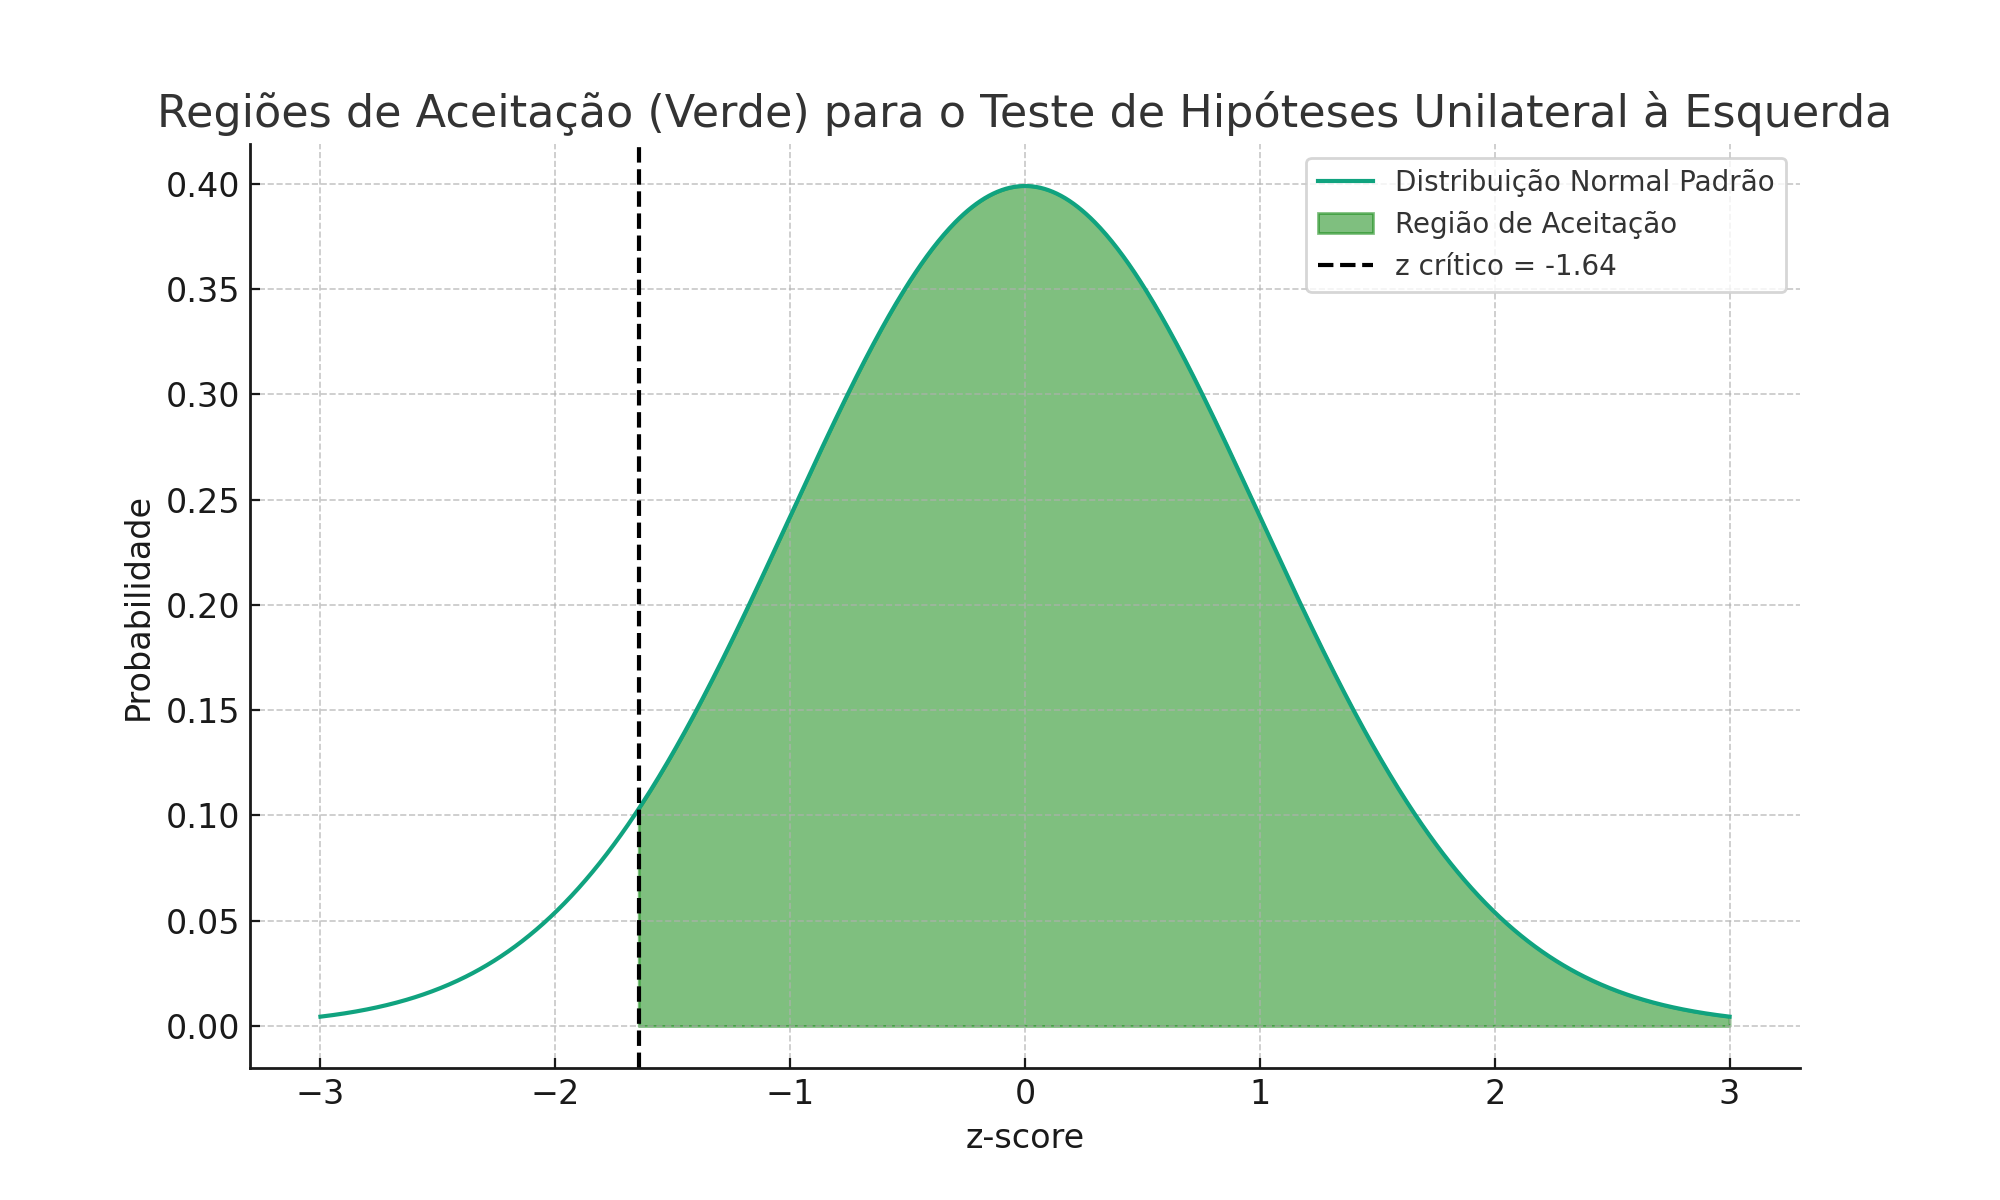
\includegraphics[scale=0.3]{ex4_plot1.png}
    \caption{Região de aceitação e região crítica em termos de $Z$.}
\end{figure}
\end{frame}
%%%%%%%%%%%%%%%%
%%%%%%%%%%%%%%%%

%%%%%%%%%%%%%%%%
% FRAME
%%%%%%%%%%%%%%%%
\begin{frame}{Exercício Nº4 -  Pág 164 de \cite{reis2021}}
\begin{itemize}
    \item{Para um valor de $\bar{X}=290<\bar{X}_C=296.71$ rejeita-se $H_0$.}
    \pause
\end{itemize}
\begin{figure}
    \centering
    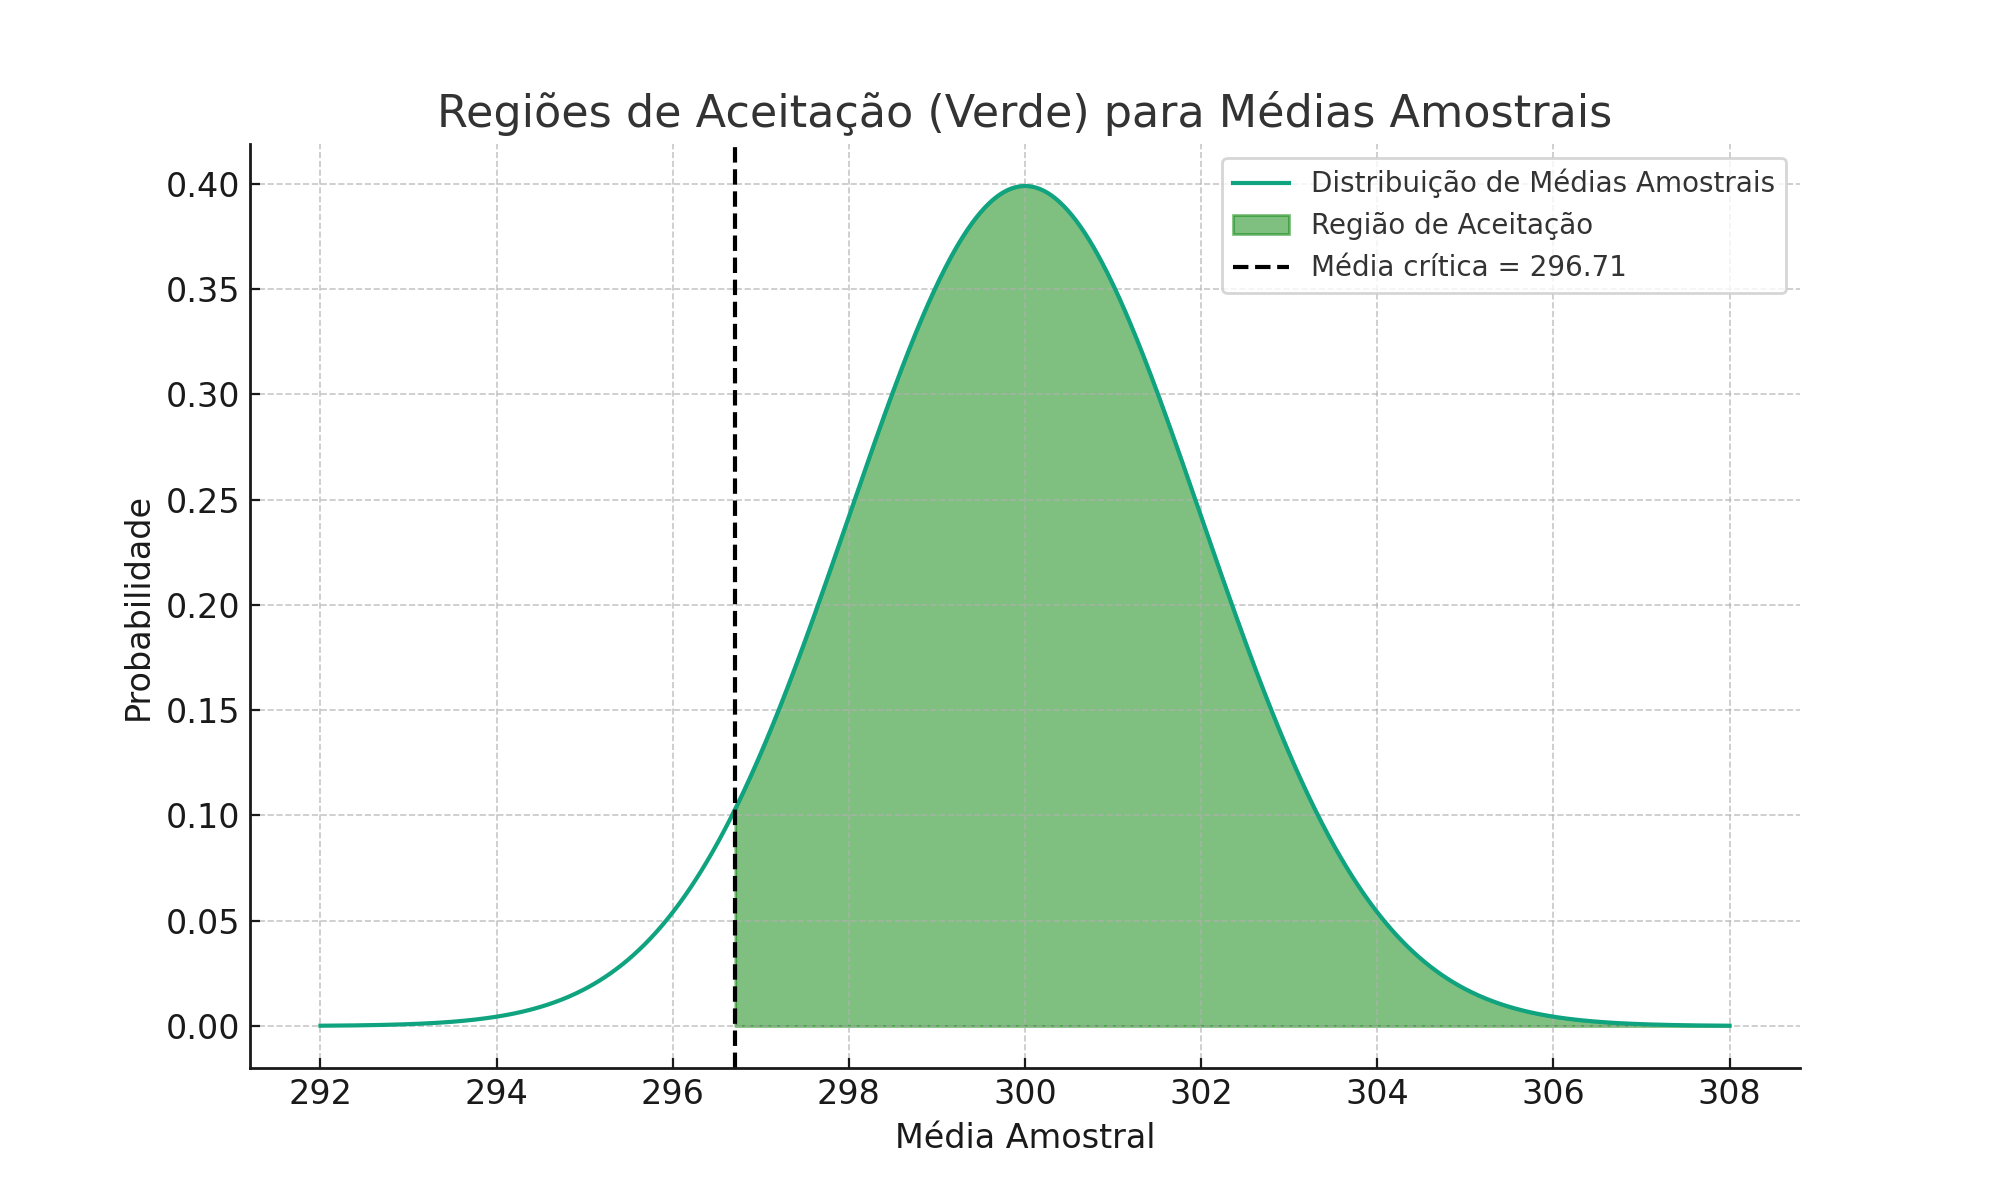
\includegraphics[scale=0.3]{ex4_plot2.png}
    \caption{Região de aceitação e região crítica em termos da média amostral $\bar{X}$.}
\end{figure}
\end{frame}
%%%%%%%%%%%%%%%%
%%%%%%%%%%%%%%%%

\section{Ex. Nº8}\label{sec:ex8}
%%%%%%%%%%%%%%%%
% FRAME
%%%%%%%%%%%%%%%%
\begin{frame}{Exercício Nº8 (a) - Pág 164 de \cite{reis2021}}
\begin{itemize}
\item{''No exame de Estatística efectuado na 2ª época no ano lectivo de 2000/2001, foram avaliados 31 alunos. Considerando este alunos como uma amostra representativa da população dos alunos matriculados na cadeira de Estatística e tendo em conta que, para essa amostra, se obtiveram os seguintes resultados:''}
\pause
\item{$\sum_{i=1}^{n=31}X_i=299$ e $\sum_{i=1}^{n=31}(X_i-\bar{X})^2=120$}
\pause
\item{''Comente a afirmação:A média dos resultados não difere significativamente de 10. Utilize $\alpha=0.05$''}
\pause
\item{Seja $X\equiv$ resultados em estatística dos alunos matriculados nesta cadeira.}
\pause
\item{Admitindo que $X\sim \mathcal{N}(\mu, \sigma)$.}
\item{Para o problema em causa as hipóteses a considerar são as seguintes:}
\item{$H_0:\mu=10$ VS $H_1:\mu\neq10$ - Ensaio bilateral para uma média de população normal com variância desconhecida.}
\end{itemize}
\end{frame}
%%%%%%%%%%%%%%%%
%%%%%%%%%%%%%%%%


%%%%%%%%%%%%%%%%
% FRAME
%%%%%%%%%%%%%%%%
\begin{frame}{Exercício Nº8 (a) - Pág 164 de \cite{reis2021}}
\begin{itemize}
\item{Tendo em consideração os dados que temos a estatística de teste é:}
\pause
\begin{equation}
    T=\frac{\bar{X} - \mu_0}{\frac{S}{\sqrt{n}}}\sim \mathcal{N}(0,1).
\end{equation}
\pause
\item{A amostra é grande $(n>30)$ - Não é necessário o $S'$.}
\end{itemize}
\pause
\begin{figure}
    \centering
    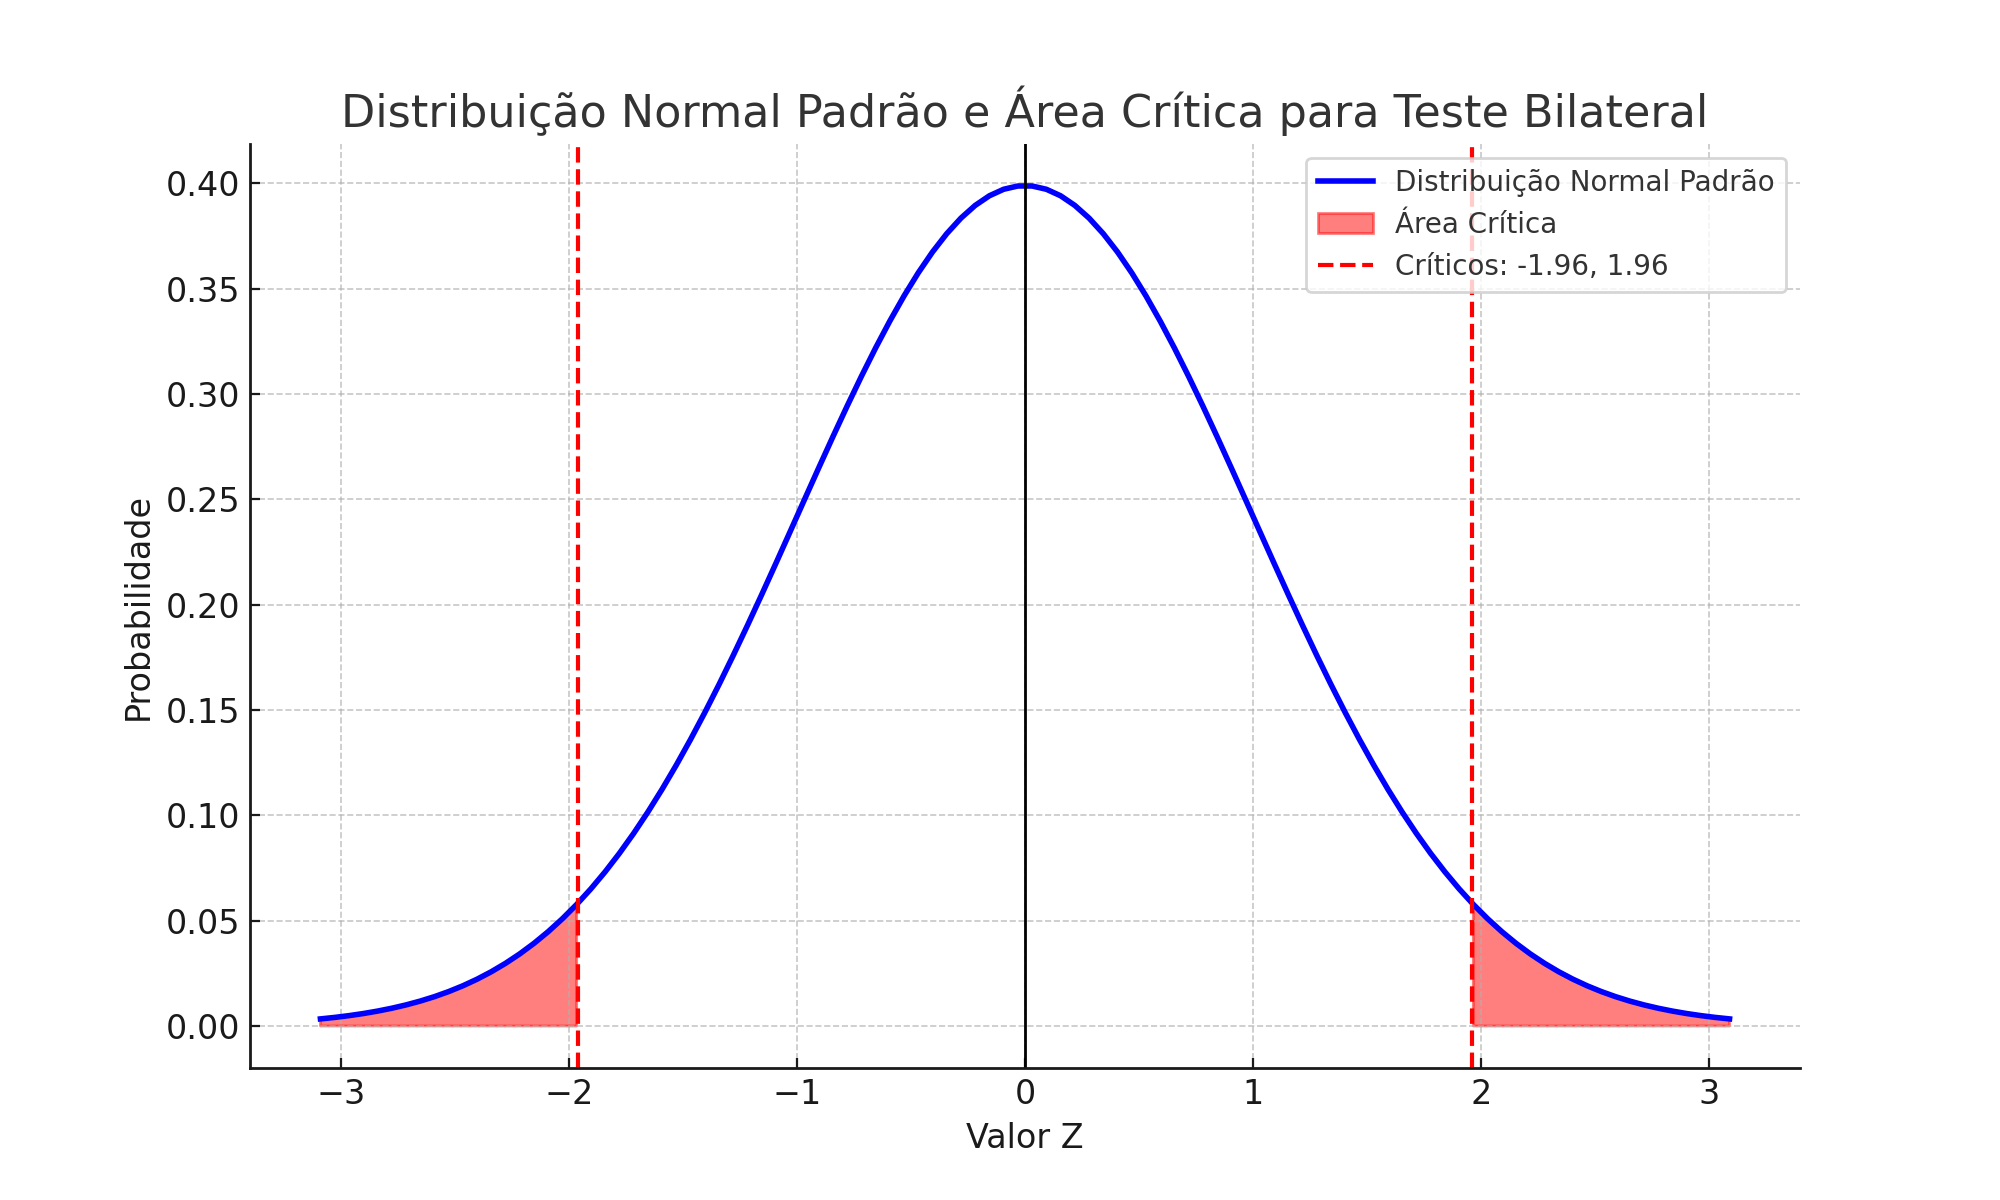
\includegraphics[scale=0.3]{corrected_normal_distribution.png}
    \caption{Região de aceitação e região crítica em termos de $Z$.}
\end{figure}
\end{frame}
%%%%%%%%%%%%%%%%
%%%%%%%%%%%%%%%%


%%%%%%%%%%%%%%%%
% FRAME
%%%%%%%%%%%%%%%%
\begin{frame}{Exercício Nº8 (a) - Pág 164 de \cite{reis2021}}
\begin{itemize}
\item{Então a região crítica e a região de aceitação são dados por, respectivamente:}
\pause
\item{R.C:$]-\infty, -1.96]\cup [+1.96, +\infty[$ e R.A:$]-1.96 , +1.96[$}
\pause
\item{Antes de calcular o valor do teste temos de fazer os seguintes cálculos:}
\pause
\item{$\bar{X}=\frac{1}{n}\cdot\sum_{i=1}^{n}X_i=\frac{1}{31}\cdot299=9.65$}
\pause
\item{$S=\sqrt{S^2}=\sqrt{\frac{1}{n}\cdot\sum_{i=1}^{n=31}(X_i-\bar{X})^2}=\sqrt{\frac{1}{31}\cdot120}=1.97$}
\pause
\item{Então o valor da estimativa para a estatística de teste é dado por:}
\pause
\end{itemize}
\begin{equation}
T^*=\frac{9.65-10}{\frac{1.97}{\sqrt{31}}}=\frac{-0.35}{0.3534}=0.9904    
\end{equation}
\begin{itemize}
    \item{Pelo que a $T^*\in$ R.A pelo que não rejeitamos $H_0$ para $\alpha=0.05$ e para esta amostra. Pelo que a afirmação é suportada pelos dados.} 
\end{itemize}
\end{frame}
%%%%%%%%%%%%%%%%
%%%%%%%%%%%%%%%%

\section{Ex. Outputs}\label{sec:outputs}
%%%%%%%%%%%%%%%%
% FRAME
%%%%%%%%%%%%%%%%
\begin{frame}[allowframebreaks]{Exercícios de Outputs - Folhas SPSS Parte II}
\begin{itemize}
    \item{Continuamos na nossa base de dados dos jornais semanais e vamos pedir umas estatísticas sobre a variável tempo de leitura}
\end{itemize}
\begin{figure}
    \centering
    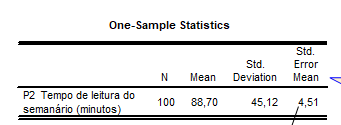
\includegraphics[scale=0.6]{p2_descritiva.png}
    \caption{Teste T unilateral e bilateral para $\mu_0=60$.}
    \label{fig:t-test}
\end{figure}
\begin{itemize}
    \item{Estamos a fazer um teste T unilateral e bilateral para a média populacional da variável tempo de leitura.} 
    \begin{itemize}
        \item{Ou seja, estamos a testar se $\mu\leq60$ ou $\mu>60$.}
        \item{Ou seja, estamos a testar se $\mu=60$ ou $\mu\neq60$.}
    \end{itemize}
\end{itemize}
\begin{figure}
    \centering
    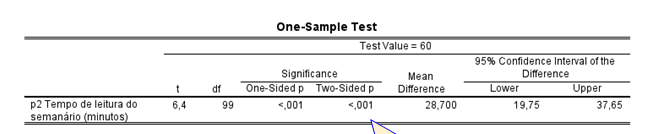
\includegraphics[scale=0.6]{teste_t_uni_bi_spss.png}
    \caption{Teste T unilateral e bilateral para $\mu_0=60$.}
    \label{fig:t-test}
\end{figure}
\begin{itemize}
    \item{A estatística de teste adequada para o dados disponíveis é:}
    \begin{equation}
        T=\frac{\bar{X}-\mu_0}{\frac{S'}{\sqrt{n}}}\sim t(n-1)
    \end{equation}
    \item{O teste está a ser realizado com uma significância de 5\% pelo que os valores critico da t-student são dados por: $\pm1.660$ and $\pm1.1984$.}
    \item{O valor de T para a amostra concreta (i.e. $T^*=6.361$) ultrapassa largamente qualquer um dos valores pelo que rejeita-se $H_0$.}
    \item{Outra maneira de se ver isto é pelo p-value associado a cada teste.}
    \item{Ambos os p-values são inferiores a 5\% pelo que $H_0$ deve ser rejeitada.}
    \item{Estamos a assumir que a amostra provém de uma população normal com variância desconhecida.}
    \item{Isto pode não ser verdade e deve ser testado - Verificar com o Kolmogorov-Smirnov.}
\end{itemize}
\end{frame}
%%%%%%%%%%%%%%%%
%%%%%%%%%%%%%%%%








%%%%%%%%%%%%%%%%
%REFERENCES 
%%%%%%%%%%%%%%%%

\begin{frame}[allowframebreaks]{References}
\nocite{*}
\bibliographystyle{plainnat}
\bibliography{aulas_de_teste_de_hipoteses.bib}
\end{frame}


%%%%%%%%%%%%%%%%%%%%%%
\end{document}
%%%%%%%%%%%%%%%%%%%%%%
